\documentclass[11pt, oneside]{article} 
\usepackage{geometry}
\geometry{letterpaper} 
\usepackage{graphicx}
	
\usepackage{amssymb}
\usepackage{amsmath}
\usepackage{parskip}
\usepackage{color}
\usepackage{hyperref}

\graphicspath{{/Users/telliott/Github/calculus_book/png/}}
% \begin{center} 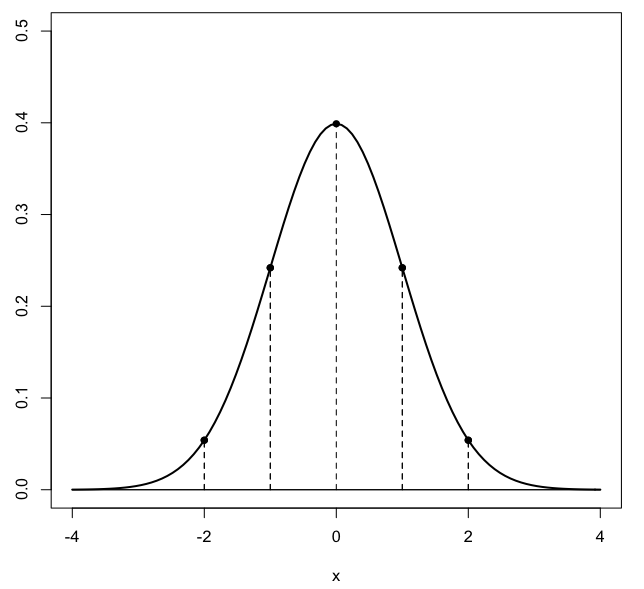
\includegraphics [scale=0.4] {gauss3.png} \end{center}

\title{Circles and ellipses}
\date{}

\begin{document}
\maketitle
\Large

A circle can be defined as all the points at the same distance from a central point, let us label that point $(h,k)$.  The distance from the points to the center is the radius, denoted $r$.

Using the Pythagorean theorem, we can calculate the square of the distance from the origin as
\[ r^2 = (x - h)^2 + (y - k)^2 \]

The simplest circles are those whose central point is the origin of the coordinate system.  In that case the equation  simplifies to 
\[ r^2 = x^2 + y^2 \]
Usually, we know the value of $r$ and we want to write an equation for $y$ in terms of $x$.  Then
\[ y^2 = r^2 - x^2 \]
\[ y = \sqrt{r^2 - x^2} \]

\subsection*{intersection of line and circle}
If we have a circle of radius $2$:
\[ x^2 + y^2 = 2 \]
and consider the line with $y$-intercept equal to $0$ and slope equal to $-1$:
\[ y = -x \]
\begin{center} 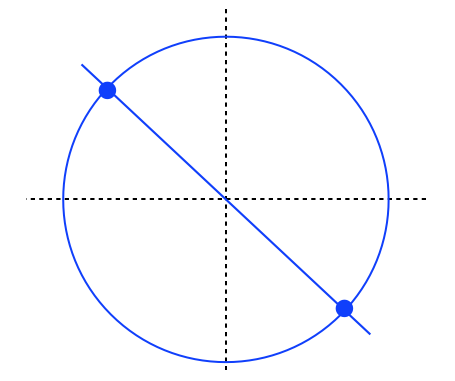
\includegraphics [scale=0.4] {line_circle.png} \end{center}

We can solve for the points where the line and the circle intersect by requiring that both equations be satisfied simultaneously:
\[ x^2 + (-x)^2 = 2 \]
\[ 2x^2 = 2 \]
\[ x =  \pm 1 \]
\[ (x,y) = (1,-1), (-1,1) \]

The symmetry is apparent.

\subsection*{tangent to the circle}

Suppose we have a unit circle and an external point $(x,y)$.  We wish to find the equation of the tangent line to a point on the circle.  Call that point $(a,b)$.

Circles are special.  The tangent line is \emph{perpendicular} to the radius at the point of tangency.

\begin{center} 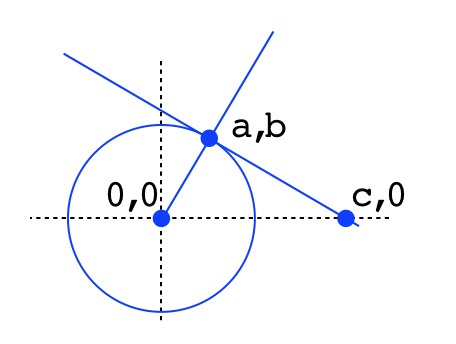
\includegraphics [scale=0.4] {tangent4.png} \end{center}

The line through $(a,b)$ and the origin has slope $b/a$ since
\[ m = \frac{b - 0}{a - 0} \]

If we have two lines with slopes $m_1$ and $m_2$ and they are perpendicular, the product $m_1m_2$ is $-1$.  So the tangent to the circle at $(a,b)$ has slope $-a/b$ and from the slope-intercept equation the tangent line through $(a,b)$ is
\[ y = -\frac{a}{b} x + y_0 \]

We need a value for the $y$-intercept or $x$-intercept.  If we can determine the value of $c$ above, we would have (at $y = 0$):
\[ 0 = -\frac{a}{b} c + y_0 \]
\[ y_0 = \frac{ac}{b} \]

Recall from the chapter on the Pythagorean theorem that the altitude squared is equal to the product of the parts of the base.  Dropping an altitude from $(a,b)$ (red line):
\[ b^2 = a(c-a) \]
\[ b^2 = ac - a^2 \]
\[ ac = 1 \]
\[ c = \frac{1}{a} \]

Plugging in:
\[ y_0 = \frac{ac}{b} \]
\[ y_0 = \frac{1}{b} \]
which we could probably predict from symmetry.
\begin{center} 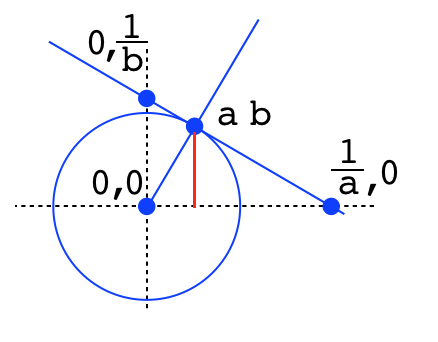
\includegraphics [scale=0.4] {tangent5.png} \end{center}

Just check the distances 
\[ \frac{1}{a^2} = a^2 + b^2 + (\frac{1}{a} - a)^2 + b^2 \]
\[ \frac{1}{a^2} = a^2 + b^2 + \frac{1}{a^2} - 2 + a^2 + b^2 \]
which looks good, when we recall that $a^2 + b^2 = 1$.

So finally
\[ y = -\frac{a}{b} x + \frac{1}{b} \]
\[ ax + by = 1 \]
a line with slope $-a/b$ whose $y$-intercept is $1/b$.

\subsection*{ellipse}
I found a problem on the web that extends this to the ellipse:

\url{https://math.stackexchange.com/questions/834392/equations-of-lines-tangent-to-an-ellipse}

In working that problem, I ended up with a quartic equation (fourth power).  This is, quite literally, a mess.

Here's a great idea for ellipse problems:  Stretch and rescale the problem to one involving a circle, by using a \emph{change of variable}.  Suppose the ellipse is
\[ \frac{x^2}{a^2} + \frac{y^2}{b^2} = 1 \]
Let $x = au$ and $y = bv$.  Then
\[ \frac{a^2u^2}{a^2} + \frac{b^2 v^2}{b^2} = 1 \]
\[ u^2 + v^2 = 1 \]

The ellipse has become a unit circle!

Apply the same transformation to any points in the problem, solve the problem, and then reverse the transformation.


\end{document}